%% LaTeX Beamer presentation template (requires beamer package)
%% see http://bitbucket.org/rivanvx/beamer/wiki/Home
%% idea contributed by H. Turgut Uyar
%% template based on a template by Till Tantau
%% this template is still evolving - it might differ in future releases!

\documentclass{beamer}

\mode<presentation>
{
	\usetheme{Warsaw}
	\usecolortheme{seahorse}
	\setbeamertemplate{footline}[frame number]
% 	\setbeamercovered{transparent}
}

\usepackage{ctex}

\usepackage{graphics}
\usepackage[ruled, vlined, boxed]{algorithm2e}

\newcommand{\set}[1]{\left\{\,#1\,\right\}}  % set {}

% for tikz
\usepackage{tikz, adjustbox}
\usetikzlibrary{positioning, shapes, arrows, snakes, mindmap, shadows,
backgrounds, fit}

\title{Time Complexity}
\subtitle{NP and NP-Complete}

\author{Hengfeng Wei}

\institute[Universities of]
{
	Institute of Computer Software, NJU
}

\date{\today}


% If you have a file called "university-logo-filename.xxx", where xxx
% is a graphic format that can be processed by latex or pdflatex,
% resp., then you can add a logo as follows:

% \pgfdeclareimage[height=0.5cm]{university-logo}{university-logo-filename}
% \logo{\pgfuseimage{university-logo}}



% Delete this, if you do not want the table of contents to pop up at
% the beginning of each subsection:
\AtBeginSubsection[]
{
	\begin{frame}<beamer>
		\frametitle{Outline}
		\tableofcontents[currentsection]
	\end{frame}
}

\AtBeginSection[]
{
	\begin{frame}<beamer>
		\frametitle{Outline}
		\tableofcontents[currentsection]
	\end{frame}
}
% If you wish to uncover everything in a step-wise fashion, uncomment
% the following command:

%\beamerdefaultoverlayspecification{<+->}

\begin{document}
%%%%%%%%%%%%%%%%%%%%%%%%%%%%%%%%%

\section{One More Dynamic Programming}

\begin{frame}
  \frametitle{RNA Secondary Structure}
  
  \begin{columns}
    \column{0.50\textwidth}
	  \begin{figure}[htp]
	  	\begin{center}
	  	  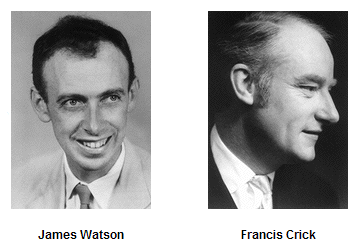
\includegraphics[width=1.00\textwidth]{figure/watson_and_crick.png}
	      \caption[labelInTOC]{Watson and Crick}
		\end{center}
	  \end{figure}    
    \column{0.50\textwidth}
	  \begin{figure}[htp]
	  	\begin{center}
	  	  
\includegraphics[width=0.60\textwidth]{figure/dna.jpg}
		\end{center}
	  \end{figure}
  \end{columns}

\end{frame}

\begin{frame}
  \frametitle{RNA Secondary Structure}

  RNA:
  \begin{columns}
    \column{0.40\textwidth}
	  \begin{figure}[htp]
	  	\begin{center}
	  	  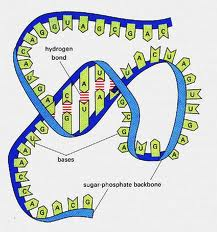
\includegraphics[width=0.80\textwidth]{figure/rna.jpg}
		\end{center}
	  \end{figure}    
    \column{0.60\textwidth}
	  \begin{figure}[htp]
	  	\begin{center}
	  	  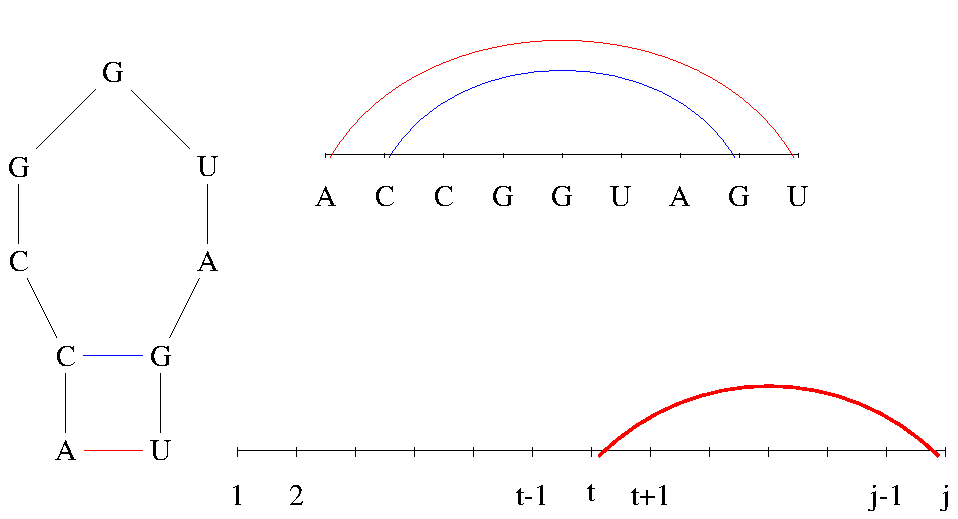
\includegraphics[width=1.00\textwidth]{figure/rna.pdf}
		\end{center}
	  \end{figure}
  \end{columns}
  
\end{frame}

\begin{frame}
  \frametitle{RNA Secondary Structure}
  
  \begin{definition}[RNA Secondary Structure]
    Alphabet: $B = \set{A, C, G, U}$
    
    RNA String: $R = b_1 b_2 \ldots b_n; b_i \in B$
    
    Secondary structure of $R$: $S = \set{(i,j)}$
    \begin{enumerate}
      \item $\forall s \in S, s \in {(A, U), (U, A), (C, G), (G, C)}$��
      \item (No sharp turns)$\forall (i,j) \in S, i < j - 4$��
      \item $S$ is a matching
      \item (Noncrossing) $\forall (i,j), (k,l) \in S, \neg(i < k
    < j < l)$��
    \end{enumerate}
    
    \[
      \textcolor{blue}{Goal: \max(\mid S \mid).}
    \]
  \end{definition}
  
\end{frame}

\begin{frame}
  \frametitle{RNA Secondary Structure}
  
  $P(i,j)$: the maximum number of pairs on $b_i \ldots b_j$.
  \[
    P(i,j) = 0, i \le j - 4; P(1,n)
  \]
  \begin{itemize}
    \item $j$ is not involved in a pair, \emph{or}
    \item $j$ pairs with $t$ for some $t < j-4$.
  \end{itemize}
  \[
    \textcolor{blue}{P(i, j) = \max \big( P(i, j-1), \max_{t:(1),(2)} (1 + P(i,
    t-1) + P(t+1, j-1)) \big).}
  \]
\end{frame}

\begin{frame}
  \frametitle{RNA Secondary Structure}

  \begin{figure}[htp]
	\begin{center}
	  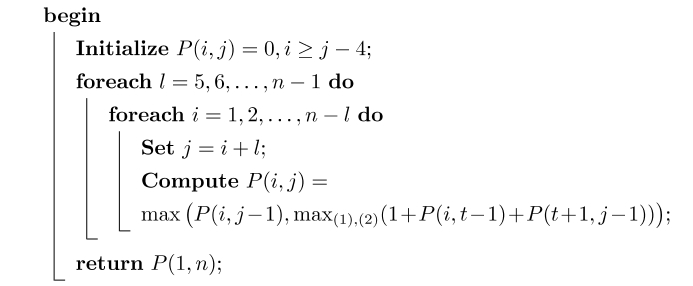
\includegraphics[width=1.00\textwidth]{figure/rnaalg.jpg}
	\end{center}
  \end{figure}
  
\end{frame}
%%%%%%%%%%%%%%%%%%%%%%%%%%%%%%%%%
\section{P and NP}

%%%%%%%%%%%%%
\begin{frame}
  \frametitle{Computability vs. Complexity Theory}
  
  Computability first:
  \begin{columns}
    \column{0.50\textwidth}
      \begin{figure}[htp]
		\begin{center}
	  	  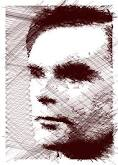
\includegraphics[width=0.50\textwidth]{figure/Turing.jpg}
		\end{center}
      \end{figure}
      \textcolor{blue}{Halting problem is undecidable.}
    \column{0.50\textwidth}
      \begin{figure}[htp]
		\begin{center}
	  	  
\includegraphics[width=0.70\textwidth]{figure/Escher.jpg}
		\end{center}
      \end{figure}
  \end{columns}

\end{frame}

%%%%%%%%%%%%%
\begin{frame}
  \frametitle{Computability vs. Complexity Theory}
  
  Complexity to follow:
  \begin{columns}
    \column{0.50\textwidth}
      \begin{figure}[htp]
		\begin{center}
	  	  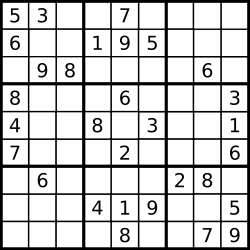
\includegraphics[width=0.60\textwidth]{figure/Sudoku.png}
		\end{center}
		\vspace{0.50cm}
		\textcolor{blue}{Easy? It is NP-Complete.}
      \end{figure}
    \column{0.50\textwidth}
      \begin{figure}[htp]
		\begin{center}
	  	  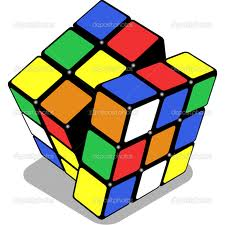
\includegraphics[width=0.60\textwidth]{figure/Rubik.jpg}
		\end{center}
      \end{figure}
      \textcolor{blue}{Hard? God's Number is 20.}
  \end{columns}
    
\end{frame}

%%%%%%%%%%%%%
\begin{frame}
  \frametitle{P vs. NP}
  
  \begin{definition}[The Class P]
    Problems decidable in polynomial time.
  \end{definition}
  
  \vspace{0.50cm}
  
  \begin{columns}
    \column{0.40\textwidth}
      \begin{itemize}
	    \setlength{\itemsep}{0.30cm}
	    
	    \item P to the input size
	    \item closed property
	    \item $\approx$ realistically efficient  
      \end{itemize}
    \column{0.60\textwidth}
      \pause
      \begin{figure}[htp]
		\begin{center}
	  	  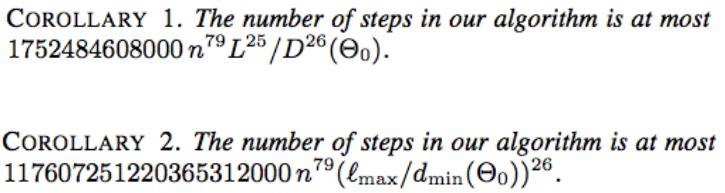
\includegraphics[width=1.0\textwidth]{figure/constant.jpg}
		\end{center}
      \end{figure}    
  \end{columns}
  
\end{frame}

%%%%%%%%%%%%%
\begin{frame}
  \frametitle{P vs. NP}

  \begin{example}[The Class P]
    \begin{columns}
      \column{0.30\textwidth}
        Euler path��
    	\begin{figure}[htp]
		  \begin{center}
		  	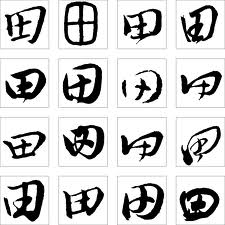
\includegraphics[width=0.80\textwidth]{figure/tian.jpg}
		  \end{center}
    	\end{figure}      
      \column{0.40\textwidth}
        Reachability:
	    \begin{figure}[htp]
		  \begin{center}
		  	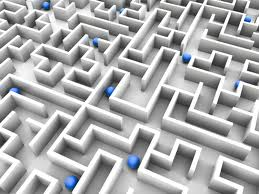
\includegraphics[width=0.80\textwidth]{figure/reachability.jpg}
		  \end{center}
	    \end{figure}      
      \column{0.30\textwidth}
        GCD:
	    \begin{figure}[htp]
		  \begin{center}
		  	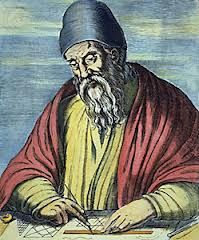
\includegraphics[width=0.70\textwidth]{figure/Euclid.jpg}
		  \end{center}
	    \end{figure}         
    \end{columns}     
  \end{example}
  
\end{frame}

%%%%%%%%%%%%%
\begin{frame}
  \frametitle{P vs. NP}
  
  \begin{example}[not \emph{known} to be in P]
    \begin{columns}
      \column{0.30\textwidth}
        Hamiltonian path:
	    \begin{figure}[htp]
		  \begin{center}
		  	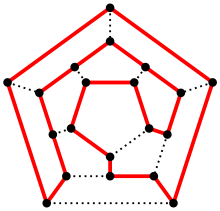
\includegraphics[width=0.80\textwidth]{figure/Hamiltonian.png}
		  \end{center}
	    \end{figure}      
      \column{0.40\textwidth}
        Clique:
	    \begin{figure}[htp]
		  \begin{center}
		  	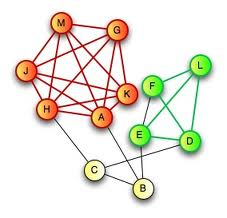
\includegraphics[width=0.70\textwidth]{figure/clique.jpg}
		  \end{center}
	    \end{figure}        
      \column{0.30\textwidth}
        Subset sum:
	    \begin{figure}[htp]
		  \begin{center}
		  	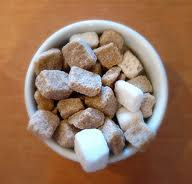
\includegraphics[width=0.80\textwidth]{figure/subset_sum.jpg}
		  \end{center}
	    \end{figure}
    \end{columns}
  \end{example}
  
  \pause
  \vspace{0.20cm}
  
  {\large \textcolor{blue}{avoiding brute force without success}}
\end{frame}

%%%%%%%%%%%%%
\begin{frame}
  \frametitle{P vs. NP}

  \begin{definition}[The Class NP]
    Problems decidable in polynomial time by \textcolor{blue}{nondeterministic}
    algorithm.
    \pause
    \[
      NP \neq \textrm{\textcolor{red}{N}on-\textcolor{red}{P}olynomial}
    \]
    \[
      NP \neq \textrm{\textcolor{red}{N}o \textcolor{red}{P}roblem}
    \]
  \end{definition}
%   
%   \pause
%   \vspace{0.50cm}
%   
%   \begin{example}[Prove]
%     \begin{enumerate}
%       \item 
%     \end{enumerate}
%   \end{example} 
\end{frame}

%%%%%%%%%%%%%
\begin{frame}
  \frametitle{P vs. NP}

  \begin{example}[Hamiltonian path $\in$ NP]
    \textcolor{blue}{Input:} $<G, s, t>$
    
    \textcolor{blue}{Problem:} Is there Hamiltonian path between $s$ and $t$ ?
  \end{example}
  
  \begin{proof}
    \begin{enumerate}
      \item select $n$ vertices, $v_1, \ldots, v_n$
        \textcolor{blue}{nondeterministically}
      \item repetition ? \emph{reject} : 2
      \item $v_1 = s, v_n = t$ ? \emph{reject} : 4
      \item $(v_i, v_{i+1}) \in E(G)$ ? \emph{accept} : \emph{reject}. 
      \item polynomial
    \end{enumerate}
  \end{proof}
\end{frame}

%%%%%%%%%%%%%
\begin{frame}
  \frametitle{P vs. NP}

  \begin{example}[Clique $\in$ NP]
    \textcolor{blue}{Input:} $<G, k>$
    
    \textcolor{blue}{Problem:} Does $G$ contain a $k$-clique?
  \end{example}
  
  \begin{proof}
    \begin{enumerate}
      \item select a subset $K \subseteq V(G)$ with size $k$
        \textcolor{blue}{nondeterministically}
      \item $\forall (K_i, K_j) \in E(G)$ ? \emph{accept} : \emph{reject}.
      \item polynomial
    \end{enumerate}
  \end{proof}
\end{frame}

%%%%%%%%%%%%%
\begin{frame}
  \frametitle{P vs. NP}

  \begin{example}[Subset sum $\in$ NP]
    \textcolor{blue}{Input:} $<S, t>$
    
    \textcolor{blue}{Problem:} Is there a subset summing to $t$ ?
  \end{example}
  
  \begin{proof}
    \begin{enumerate}
      \item select a subset $C \subseteq S$
        \textcolor{blue}{nondeterministically}
      \item $\sum C = t$ ? \emph{accept} : \emph{reject}. 
      \item polynomial
    \end{enumerate}
  \end{proof}
\end{frame}

%%%%%%%%%%%%%
\begin{frame}
  \frametitle{P vs. NP}
  
  \begin{columns}
    \column{0.50\textwidth}
	    \begin{figure}[htp]
		  \begin{center}
		  	\includegraphics[scale = 0.30]{figure/P_NP.jpg}
		  \end{center}
	    \end{figure}
	\column{0.50\textwidth}
	    \begin{figure}[htp]
		  \begin{center}
		  	
\includegraphics[scale = 0.30]{figure/x.jpg}
		  \end{center}
	    \end{figure}	    
  \end{columns}
  
  \begin{columns}
    \column{0.50\textwidth}
      \begin{itemize}
        \item P = \emph{\textcolor{blue}{decided}} quickly
        \item solving problem
        \item composing
      \end{itemize}   
    \column{0.50\textwidth}
      \begin{itemize}
        \item NP = \emph{\textcolor{blue}{verified}} quickly
        \item checking the solution
        \item appreciating symphony 
      \end{itemize}
  \end{columns}
  
\end{frame}

%%%%%%%%%%%%%
\begin{frame}
  \frametitle{P vs. NP}
  
  \begin{figure}[htp]
	\begin{center}
	  
\includegraphics[width=0.40\textwidth]{figure/wanted.jpg}
	\end{center}
  \end{figure} 
  
\end{frame}
%%%%%%%%%%%%%
\begin{frame}
  \frametitle{P vs. NP}
  
  \begin{figure}[htp]
	\begin{center}
	  
\includegraphics[width=0.50\textwidth]{figure/homor.pdf}
	\end{center}
  \end{figure} 
  
\end{frame}

%%%%%%%%%%%%%
\begin{frame}
  \frametitle{P vs. VP}
  
  \begin{quote}
    ``Milestones'' in 
    
    {\small \url{http://www.win.tue.nl/~gwoegi/P-versus-NP.htm}}
  \end{quote}
  
  \vspace{0.50cm}
  
  \begin{quote}
    It will be solved by either 2048 or 4096. (Knuth)
  \end{quote}
  
\end{frame}
%%%%%%%%%%%%%%%%%%%%%%%%%%%%%%%%%
\section{NP-Complete}

%%%%%%%%%%%%%
\begin{frame}
  \frametitle{NP-Complete}
  
  \begin{columns}
    \column{0.50\textwidth}
      \textcolor{blue}{How hard are they ?}
	  \begin{enumerate}
	    \setlength{\itemsep}{0.30cm}
	    \item Hamiltonian path
	    \item Clique
	    \item Subset sum
	  \end{enumerate}
    \column{0.50\textwidth}
	  \begin{figure}[htp]
		\begin{center}
		  
\includegraphics[width=0.60\textwidth]{figure/sad.jpg}
		\end{center}
	  \end{figure}
  \end{columns}   
\end{frame}

%%%%%%%%%%%%%
\begin{frame}
  \frametitle{NP-Complete}
  
  NP-Complete problem (\textcolor{blue}{[@1970s]}):
  \begin{enumerate}
    \setlength{\itemsep}{0.30cm}
    \item subset of $P$
    \item any problem in $NP$ \textcolor{blue}{\emph{reducible to}} any one in
    $NPC$
    \item hard core of $NP$
    \item one is polynomial $\Rightarrow$ all are polynomial 
  \end{enumerate}
  
\end{frame}

%%%%%%%%%%%%%
\begin{frame}
  \frametitle{NP-Complete}

  Key concept: polynomial time reduction
  \begin{figure}[htp]
	\begin{center}
	  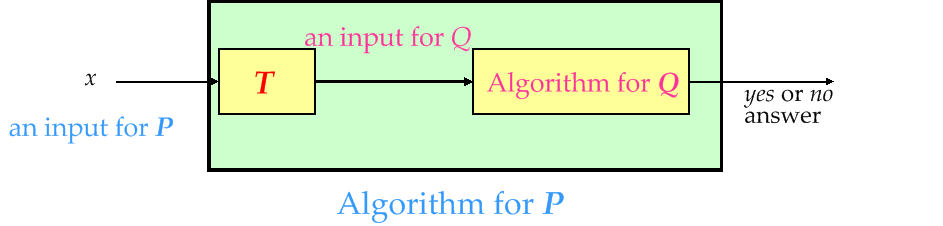
\includegraphics[width=1.00\textwidth]{figure/reduction.png}
	\end{center}
  \end{figure}  

  $P \le_{P} Q$
  \begin{itemize}
    \item \emph{difficulty} flows forward
    \item \emph{efficient} flows backward
    \item \emph{composition}
  \end{itemize}
\end{frame}

%%%%%%%%%%%%%
\begin{frame}
  \frametitle{NP-Complete}
  
  Reducibility among known problems (\textcolor{blue}{[Karp@70s]})
  \begin{figure}[htp]
	\begin{center}
	  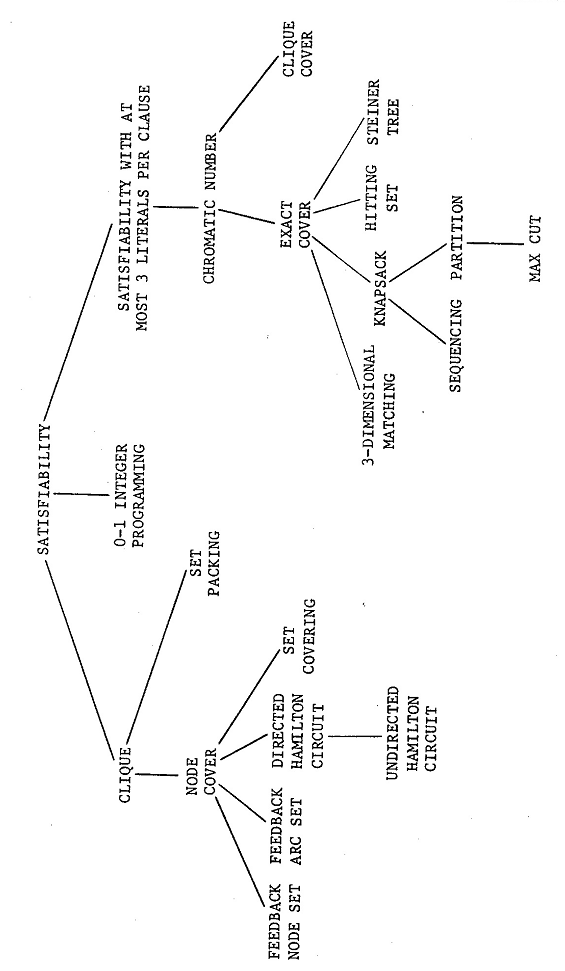
\includegraphics[scale = 0.40, angle = -90]{figure/reducibility.png}
	\end{center}
  \end{figure} 
     
\end{frame}

%%%%%%%%%%%%%
\begin{frame}
  \frametitle{NP-Complete: Known NPC Problems}
  
  1. Packing Problems:
  \begin{example}[Independent Set]
    Given a graph $G$ and a number $k$, 
    
    does $G$ contain an independent set of size $k$?
  \end{example}
  
\end{frame}

\begin{frame}
  \frametitle{NP-Complete: Known NPC Problems}
  
  1. Packing Problems:
  \begin{example}[Set Packing]
    Given a universe $\mathcal{U}$, a family $\mathcal{F}$ of subsets of
    $\mathcal{U}$ and a number $k$, 
    
    is there a subfamily $\mathcal{C} \subseteq
    \mathcal{F}$ of size $k$ such that all sets in $\mathcal{C}$ are pairwise
    disjoint?
    
    \vspace{0.30cm}
    \begin{figure}[htp]
	  \begin{center}
	    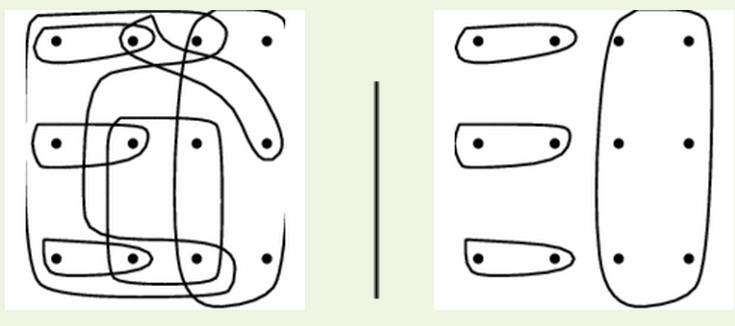
\includegraphics[width = 0.70\textwidth]{figure/setpacking.jpg}
	  \end{center}
    \end{figure} 
  \end{example}
  
\end{frame}
%%%%%%%%%%%%%
\begin{frame}
  \frametitle{NP-Complete: Known NPC Problems}
  
  2. Covering Problems:
  \begin{example}[Vetex Cover]
    Given a graph $G$ and a number $k$,
    
    does $G$ contain a vertex cover (\emph{a subset $D$ of vertices where every
    edge of $G$ touches one of those nodes}) of size $k$?
    
    \vspace{0.30cm}
    \begin{figure}[htp]
	  \begin{center}
	    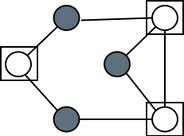
\includegraphics[width = 0.40\textwidth]{figure/vertex_cover.jpg}
	  \end{center}
    \end{figure}     
  \end{example}
  
\end{frame}

%%%%%
\begin{frame}
  \frametitle{NP-Complete: Known NPC Problems}
  
  2. Covering Problems:
  \begin{example}[Dominating Set]
    Given a graph $G$ and a number $k$,
    
    does $G$ contain a dominating set (\emph{a subset $D$ of vertices where
    every other vertex is joined to at least one member of $D$}) of size $k$?
    
    \vspace{0.30cm}
	\begin{figure}[htp]
	  \begin{center}
	  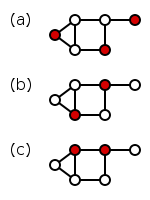
\includegraphics[width = 0.35\textwidth, angle =
	  90]{figure/dominating_set.png}
	  \end{center}
	\end{figure}      
  \end{example}
  
\end{frame}

\begin{frame}
  \frametitle{NP-Complete: Known NPC Problems}
  
  2. Covering Problems:
  \begin{example}[Set Cover]
    Given a universe $\mathcal{U}$, a family $\mathcal{F}$ of subsets of
    $\mathcal{U}$ and a number $k$, 
    
    is there a subfamily $\mathcal{C} \subseteq
    \mathcal{F}$ of size $k$ whose union is $\mathcal{U}$?
    
    \vspace{0.30cm}
    \begin{columns}
      \column{0.40\textwidth}
	    \begin{figure}[htp]
		  \begin{center}
		    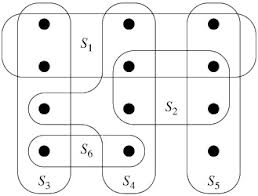
\includegraphics[width = 1.00\textwidth]{figure/set_cover.jpg}
		  \end{center}
	    \end{figure}      
      \column{0.60\textwidth}
        \[
          \mathcal{U} = \set{1, 2, 3, 4, 5}
        \]
        \[
          \mathcal{F} = \set{\set{1,2,3}, \set{2,4}, \set{3,4}, \set{4,5}}
        \]
        \[
          \textcolor{blue}{\mathcal{C} = \set{\set{1,2,3}, \set{4,5}}}
        \]
    \end{columns}
  \end{example}
  
\end{frame}
%%%%%%%%%%%%%
\begin{frame}
  \frametitle{NP-Complete: Known NPC Problems}
  
  3. Partition Problems:
  \begin{example}[Graph Coloring]
    Given a graph $G$ and a number $k$,
    
    does $G$ have a $k$-coloring ($c: V \rightarrow \set{1, \ldots, k};
    \forall (u,v) \in E, c(u) \neq c(v)$)?
    
    \vspace{0.30cm}
	\begin{figure}[htp]
	  \begin{center}
	  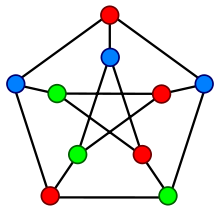
\includegraphics[width = 0.35\textwidth]{figure/3coloring.png}
	  \end{center}
	\end{figure} 
  \end{example}
\end{frame}

\begin{frame}
  \frametitle{NP-Complete: Known NPC Problems}
  
  3. Partition Problems:
  \begin{example}[3D Matching]
    Given disjoint sets $X, Y, Z$, each of size $n$, and a set $T \subseteq X
    \times Y \times Z$ of ordered triples, 
    
    does there exist a set of $n$ triples in $T$ such that each element of $X
    \cup Y \cup Z$ is contained in exactly one of these triples?
  \end{example}
\end{frame}

\begin{frame}
  \frametitle{NP-Complete: Known NPC Problems}
  
  3. Partition Problems:
  \begin{example}[3D Matching (cont.)]
    
	    \begin{figure}[htp]
		  \begin{center}
		    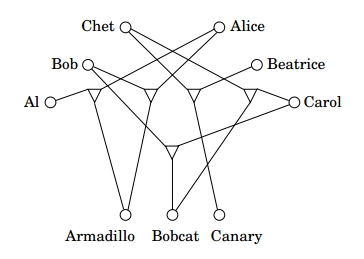
\includegraphics[width = 0.60\textwidth]{figure/3dmatching.jpg}
		  \end{center}
	    \end{figure}
	\[
	  (Al, Alice, Armadillo); (Bob, Carol, Bobcat); (Chet, Beatrice, Canary).
	\]      
  \end{example}
\end{frame}
%%%%%%%%%%%%%
\begin{frame}
  \frametitle{NP-Complete: Known NPC Problems}
  
  4. Sequencing Problems:
  \begin{example}[Hamiltonian Path]
    Given a (un)directed graph $G$ and vertices $s, t$,
    
    is there a Hamiltonian path (\emph{visiting every vertex exactly once}) between $s$ and $t$?
    
    \vspace{0.30cm}
	    \begin{figure}[htp]
		  \begin{center}
		  	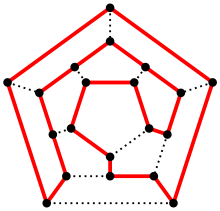
\includegraphics[width=0.30\textwidth]{figure/Hamiltonian.png}
		  \end{center}
	    \end{figure}
  \end{example}
\end{frame}

\begin{frame}
  \frametitle{NP-Complete: Known NPC Problems}
  
  4. Sequencing Problems:
  \begin{example}[Hamiltonian Cycle]
    Given a (un)directed graph $G$,
    
    is there a Hamiltonian cycle (\emph{visiting every vertex exactly once})?

    \vspace{0.30cm}
	    \begin{figure}[htp]
		  \begin{center}
		  	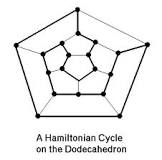
\includegraphics[width=0.40\textwidth]{figure/Hcycle.jpg}
		  \end{center}
	    \end{figure}
  \end{example}
\end{frame}

\begin{frame}
  \frametitle{NP-Complete: Known NPC Problems}
  
  4. Sequencing Problems:
  \begin{example}[Traveling Salesman Problem (TSP)]
    Given a set of distances on $n$ cities and a number $k$,
    
    is there a cycle visiting every vertex exactly once of total distance $k$
    or less?
    
    \vspace{0.30cm}
	    \begin{figure}[htp]
		  \begin{center}
		  	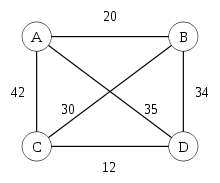
\includegraphics[width=0.40\textwidth]{figure/tsp.png}
		  \end{center}
	    \end{figure}
  \end{example}
\end{frame}
%%%%%%%%%%%%%
\begin{frame}
  \frametitle{NP-Complete: Known NPC Problems}
  
  5. Numerical Problems
  \begin{example}[Subset Sum]
    Given natural numbers $w_1, \ldots, w_n$, and a targe number $W$,
    
    is there a subset of $\set{w_1, \ldots, w_n}$ that sums to precisely $W$?
    
    \vspace{0.30cm}
    \[
      S = \set{-7, -3, -2, 5, 8}, W = 0
    \]
    \[
      \set{-3,-2,5}.
    \]
  \end{example}
\end{frame}

%%%%%%%%%%%%%
\begin{frame}
  \frametitle{NP-Complete: Known NPC Problems}
  
  6. Constraint Satisfaction Problems
  \begin{example}[3SAT]
    Given a set of clauses $C_1, \ldots, C_k$, each of length 3, over a set of
    variables $X = \set{x_1, \ldots, x_n}$,
    
    is there a satisfying truth assignment?
    
    \vspace{0.30cm}
    \[
      (x \lor y \lor z) \land (x \lor \neg y \lor z) \land (\neg x \lor \neg y
      \lor \neg z) \land (z \lor \neg x \lor y)
    \]
  \end{example}
\end{frame}
%%%%%%%%%%%%%
\begin{frame}
  \frametitle{NP-Complete}
  
  \begin{definition}[NP-Completeness proof]
    \begin{enumerate}
      \setlength{\itemsep}{0.30cm}
      \item Prove that $L \in NP$.
        \begin{itemize}
          \item Describe a nondeterministic algorithm $A$.
          \item Prove that $A$ is in polynomial time.
        \end{itemize}
      \item Select a known NP-Complete problem $L'$.
      \item Give a reduction $R$ from $L'$ to $L$.
      \item Prove that $R$ satisfies: $x' \in L' \iff x \in L$.
      \item Prove that $R$ is in polynomial time.
    \end{enumerate}
  \end{definition}
\end{frame}

%%%%%%%%%%%%%
\begin{frame}
  \frametitle{NP-Complete}

  \begin{example}[Independent Set(IS) $\rightarrow$ Vertex Cover(VC)]
    \begin{enumerate}
      \item Prove that $VC \in NP$.
      \item Reduction $R$ from $IS$ to $VC$: $(G, k) \rightarrow (G'=G, n-k)$
      \item Prove that $R$ satisfies: 
        \[
          G \textrm{ has IS with size } k (\mathcal{I}) \iff G' \textrm{ has VC
          with size } n-k (\mathcal{C})
        \]
          \begin{itemize}
            \item $\Rightarrow: \mathcal{I} \rightarrow \mathcal{C} = V -
            \mathcal{I}$.
            \item $\Leftarrow: \mathcal{C} \rightarrow \mathcal{I} = V -
            \mathcal{C}$.
          \end{itemize}
      \item Prove that $R$ is in polynomial time. Trivial.
    \end{enumerate}    
  \end{example}
\end{frame}

%%%%%%%%%%%%%
\begin{frame}
  \frametitle{NP-Complete}

  \begin{example}[Independent Set(IS) $\rightarrow$ Clique(CQ)]
    \begin{enumerate}
      \item Prove that $CQ \in NP$.
      \item Reduction $R$ from $IS$ to $CQ$: $\big (G = (V,E), k \big )
      \rightarrow \big ( \bar{G} = (V, \bar{E}), k \big )$
      \item Prove that $R$ satisfies: 
        \[
          G \textrm{ has IS with size } k (\mathcal{I}) \iff G' \textrm{ has CQ
          with size } k (\mathcal{C})
        \]
          \begin{itemize}
            \item $\Rightarrow: \mathcal{I} \rightarrow \mathcal{C} = 
            \mathcal{I}$.
            \item $\Leftarrow: \mathcal{C} \rightarrow \mathcal{I} = 
            \mathcal{C}$.
          \end{itemize}
      \item Prove that $R$ is in polynomial time. Trivial.
    \end{enumerate}    
  \end{example}
\end{frame}
%%%%%%%%%%%%%%%%%%%%%%%%%%%%%%%%%
\section*{Summary}

\begin{frame}
  \frametitle{Summary}
  
  \begin{enumerate}
    \setlength{\itemsep}{0.30cm}
    \item P vs. NP
    \item NP proof
    \item Reduction
    \item NP-Complete
    \item NP-Complete proof
  \end{enumerate}
  
\end{frame}

%%%%%%%%%%%%%%%%%%%%%%%%%%%%%%%%%%
\end{document}
